\begin{figure}[h]
	\centering
	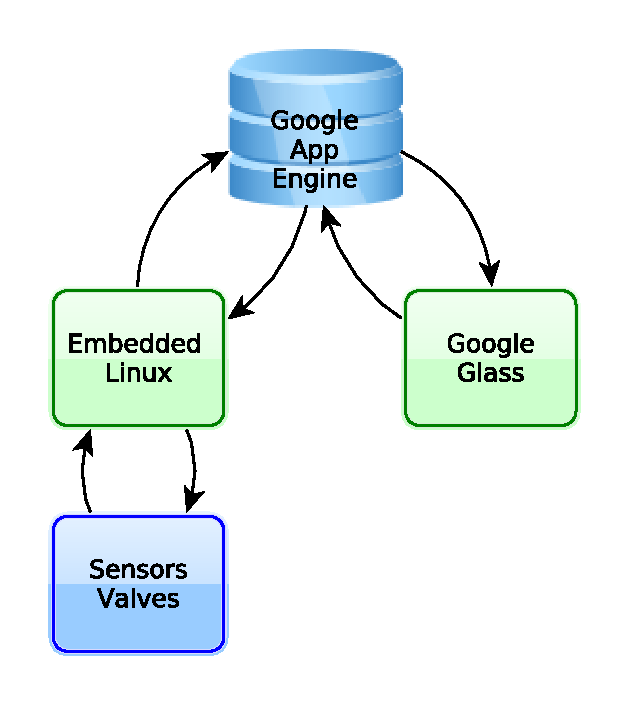
\includegraphics[scale = .9]{bo}
	\caption{High Level System's Block Diagram}
	\label{Fig:logicalview}
	
\end{figure}

The term \textit{Embedded Systems} is widely used nowadays, because its definition is  very generic: any device that includes a programmable computer, but is not itself a general-purpose computer is referred as Embedded Systems.

Indeed this definition covers a huge number of systems, from  a vending machine to a smartphone, form a electric toothbrush to a body computer of a car.\\
Peculiarity of an Embedded System is that it has hardware and software parts, takes advantage of application characteristics to optimize the design, interacts with the external environment using sensors and actuators.

\textbf{Embedded Linux} systems are a subset of embedded systems that are enhanced by a Linux operating system (\textit{OS}), here the integration of high-level Linux software and low-level electronics represents a paradigm shift in embedded systems development \cite{EBB}. It allows an easy way to design systems that can meet future challenges in smart buildings, the Internet of Things (\textit{IoT}), human-computer interaction(\textit{HCI}), robotics, and many other applications.

In this thesis project, as can be seen from (Fig.\ref{Fig:logicalview}), the system may be intended as an \textit{IoT} one. Indeed, in order to allow the interfacing between sensors and electrovalves with the Google Glass, I had to use an Internet connection, represented by the Google App Engine. And, while the Google Glass can interact directly with this server, the hardware described in (Part.\ref{HW}) needs a micro computer to be connected with that server.

\section{A Brief Introduction To IoT} 

The term Internet of Things is broadly used to describe the extension of the web and the Internet for the physical objects or "\textit{things}". It is important to realize that the physical connection of the human Internet and the ones of the \textit{IoT} are the same. And even if the \textit{IoT} term has be coined recently, the majority of web traffic nowadays is non-human \cite{ALTIOT}.

Indeed, the massive usage of online services, in part due to the smartphone revolution, has increased the interactions between servers, machine-to-machine (\textit{M2M}) communications. This trend can only increase since it is expected an explosion of wearable systems, such as smartwatch, smartglass and so on..



\begin{figure}[h]
	\centering
	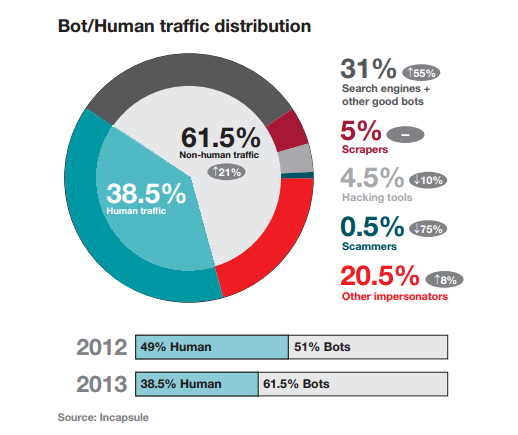
\includegraphics[scale = .65]{traffic}
	\caption{Distribution of Internet of Things}
	\label{Fig:traffic}
	
\end{figure}

In the near future, \textit{Cisco IBSG} predicts there will be $25$ billion devices connected to the Internet by $2015$ and this number is destinate to reach $50$ billion by $2020$, see (Fig.\ref{Fig:cisco})\cite{CISCOIOT}. It is also important to see that these number are based on the grown of $2011$ and do  not consider the rapid advances in device technology. So the number shown in (Fig.\ref{Fig:cisco}) have to be considered as minimum.

\begin{figure}[h]
	\centering
	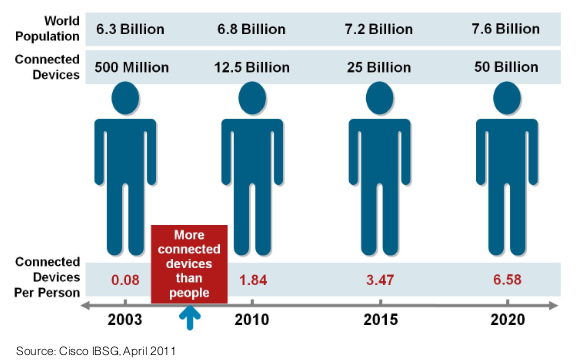
\includegraphics[scale = .65]{cisco}
	\caption{The \textit{IoT} Evolution Prediction}
	\label{Fig:cisco}
	
\end{figure}


The IoT concept, that has been exploited even in this thesis, is that if physical sensors and actuators can be linked to the Internet , then a lot of new applications and services are possible \cite{EBB}.

\section{The Beaglebone Black}

For this thesis, the Embedded Linux system has been developed using the \textit{Beaglebone Black}.\\

\begin{figure}[h]
	\centering
	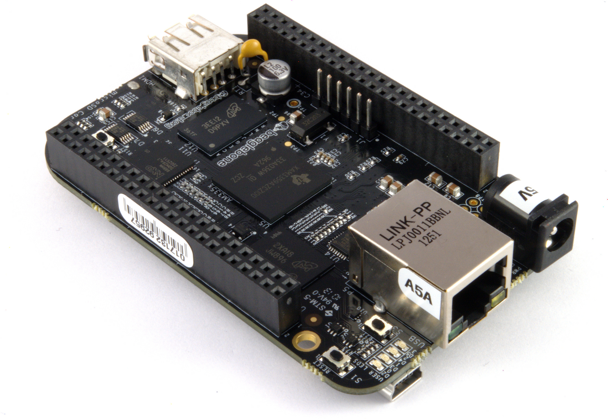
\includegraphics[scale=.55]{beaglebone}
	\caption{The \textit{Beaglebone Black}}
	\label{Fig:beaglebone}
	
\end{figure}

The \textit{Beaglebone Black} is a low-cost, fully open-source (that means everyone can downloads and uses the hardware schematics and layout in order to build up a complete product design), single board micro computer (\textit{SBC}) powered by Linux. 

There are a lot of \textit{SBC} on the market, I chose the Beaglebone Black for the following reasons:
\begin{itemize}
	\item low price, it costs $\$50 $;
	\item powerful, the \textit{Sitara\texttrademark AM335x ARM\textregistered Cortex\texttrademark-A8} processor from Texas Instruments (\textit{TI}) can run up to $1\ GHz$, allowing up to $2$ billion instructions per second;
	\item $4GB$ on-board embedded multi-media card (\textit{eMMC}), this means the Beaglebone can boot without a \textit{SD} card, unlike other boards like Raspberry PI. It allows faster boot, approximately $10$ seconds;
	\item $512MB$ \textit{DDR3} of system memory;
	\item Ethernet processor, which supports \textit{DHCP}, so it can be directly conncted to a network
	\item \textbf{expansion headers}, $92$ pins with $65$ \textit{GPIOs}, $8$ analog output, $7$ analog input, $3$ different voltage supplies ($5\ V$, $3.3\ V$, and $1.8\ V$), and the whole most used digital interface. All these make the Beaglebone Black built to be interfaced to. 
	
\end{itemize}
Over these, the board has other important feature that are not used in this thesis, but may be used in the future to enhance it. An example is given by the 2 Programmable Real-time Units (\textit{PRU}) that, unlike the definitions of Embedded Linux, make this board usable for real-time applications.

As already said in (Chap.\ref{ch:Analog}), this board has been connected to a custom \textit{capes}, a daughterboard that can be attached to the two headers on the Beaglebone itself.
